% Documento de Resultados TSP para Overleaf
% Integração com Caixeiro Viajante

\documentclass[11pt,a4paper]{article}
\usepackage[utf-8]{inputenc}
\usepackage[portuguese]{babel}
\usepackage{graphicx}
\usepackage{booktabs}
\usepackage{array}
\usepackage{float}
\usepackage{hyperref}

\title{Otimização de Rotas por TSP\\Projeto: Caixeiro Viajante}
\author{Eduardo Lopes Jonker}
\date{\today}

\begin{document}

\maketitle

\section{Resultados da Otimização de Rotas}

\subsection{Tabela 1: Comparação de Distâncias}

\begin{table}[H]
\centering
\begin{tabular}{|l|c|c|c|}
\hline
\textbf{Métrica} & \textbf{Rota Aleatória (km)} & \textbf{Rota Otimizada (km)} & \textbf{Redução (\%)} \\
\hline
Distância Total & 3501.27 & 1450.11 & 58.58\% \\
Número de Cidades & 18 & 18 & --- \\
Fator de Melhoria & 1.00x & 2.41x & --- \\
\hline
\end{tabular}
\caption{Tabela 1: Resultados do Traveling Salesman Problem (TSP)}
\label{tab:tsp_resultados}
\end{table}

\section{Visualizações}

\subsection{Mapa de Rotas Otimizadas}

A Figura~\ref{fig:mapa_master} apresenta o mapa comparativo das rotas.

\begin{figure}[H]
\centering
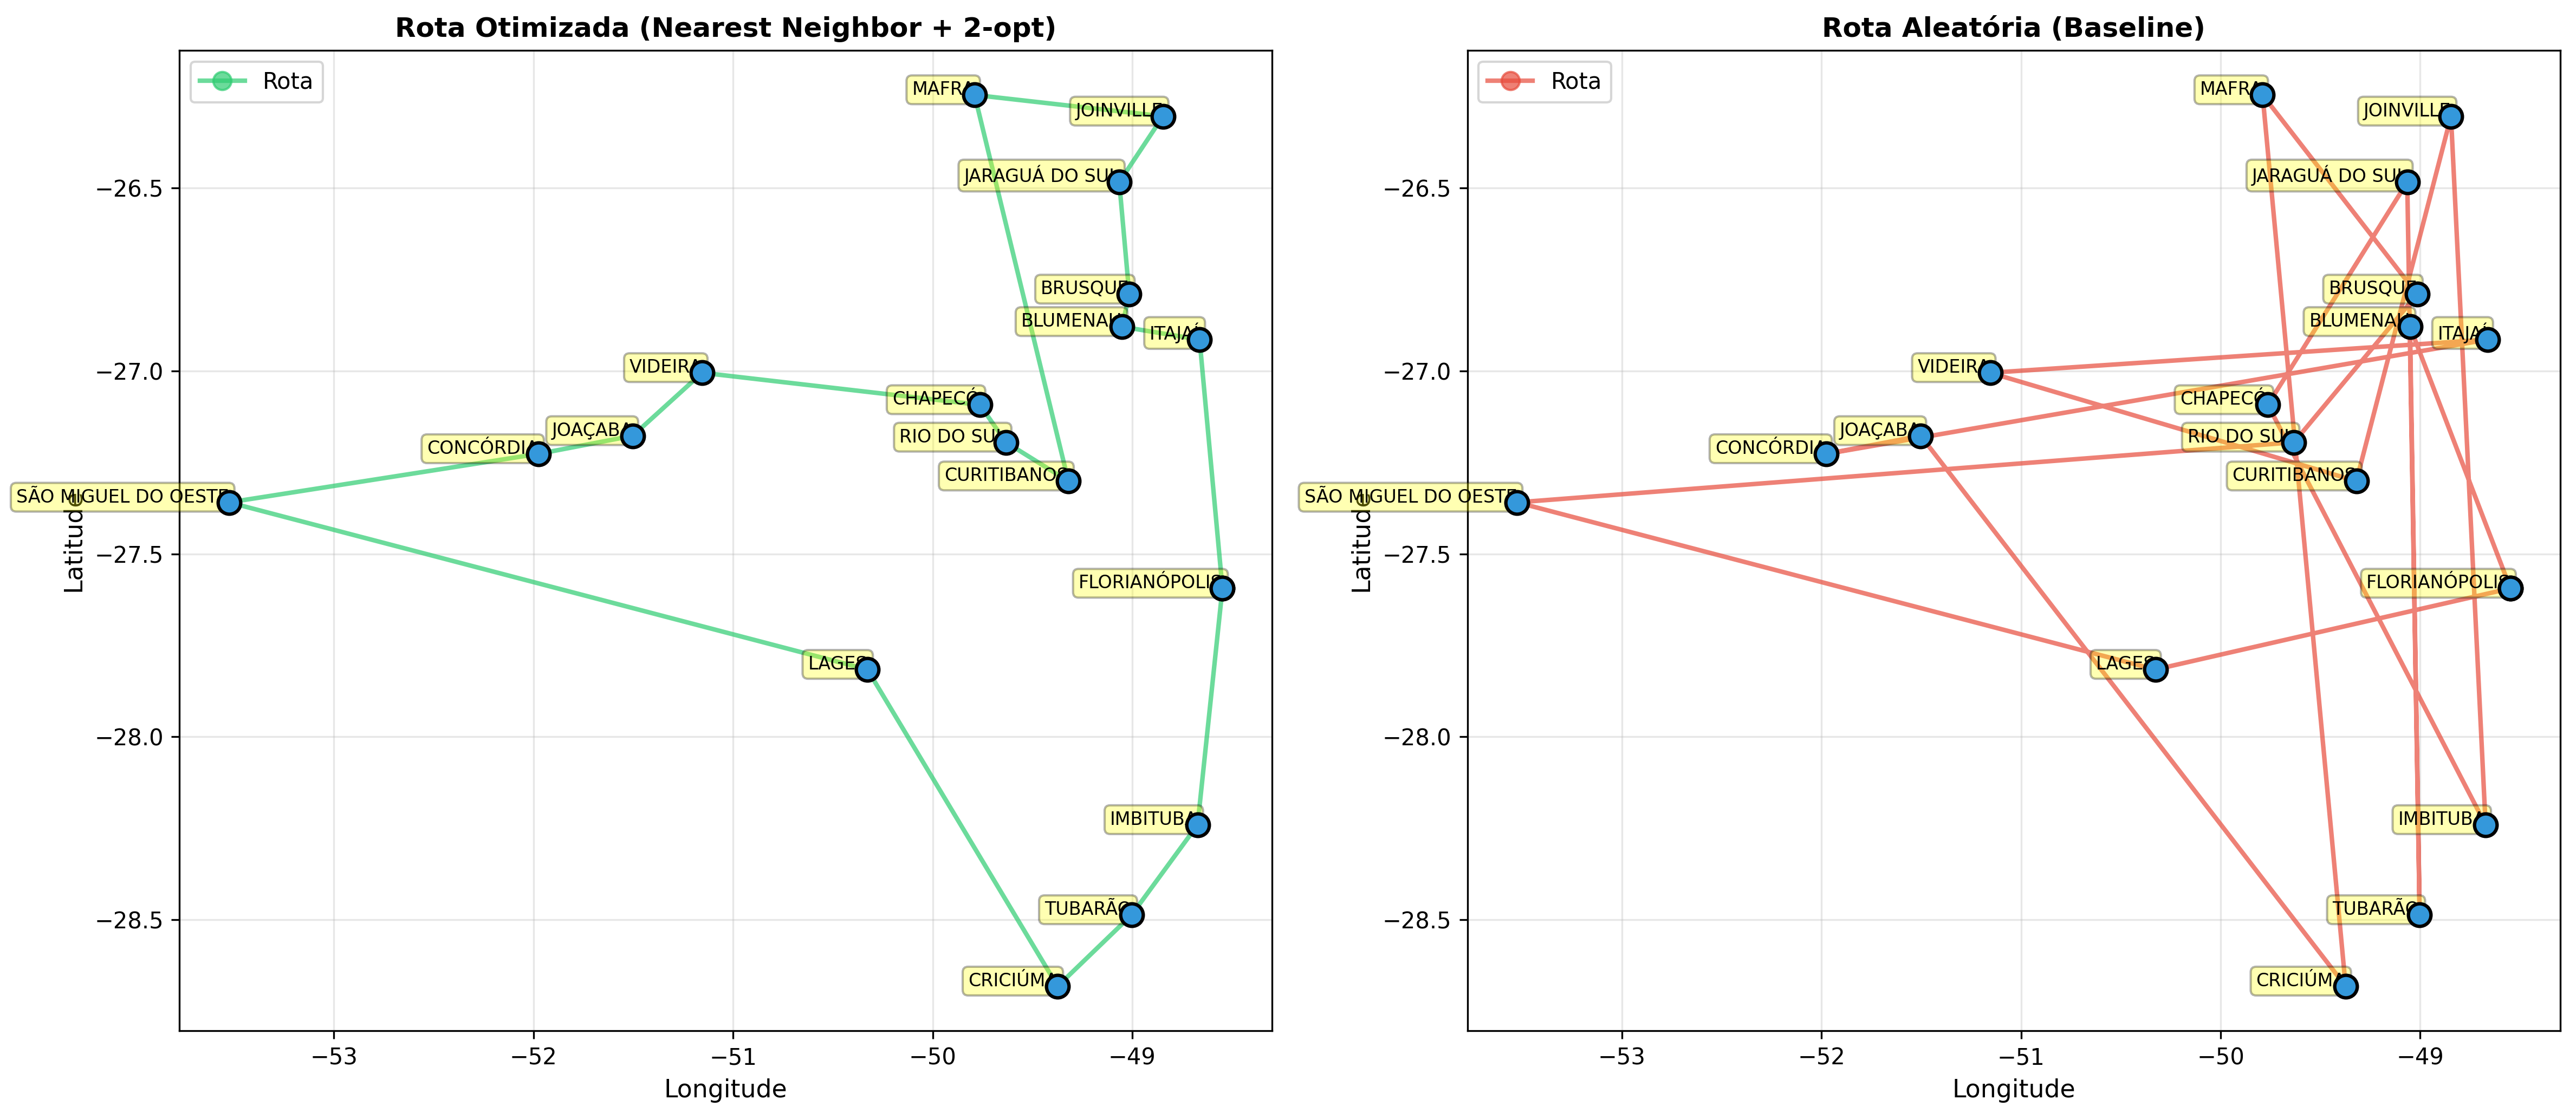
\includegraphics[width=0.9\textwidth]{mapa_master.png}
\caption{Comparação visual: Rota Otimizada (2-opt) vs Rota Aleatória}
\label{fig:mapa_master}
\end{figure}

\subsection{Gráfico Comparativo}

A Figura~\ref{fig:comparativo_master} mostra a redução de distância alcançada.

\begin{figure}[H]
\centering
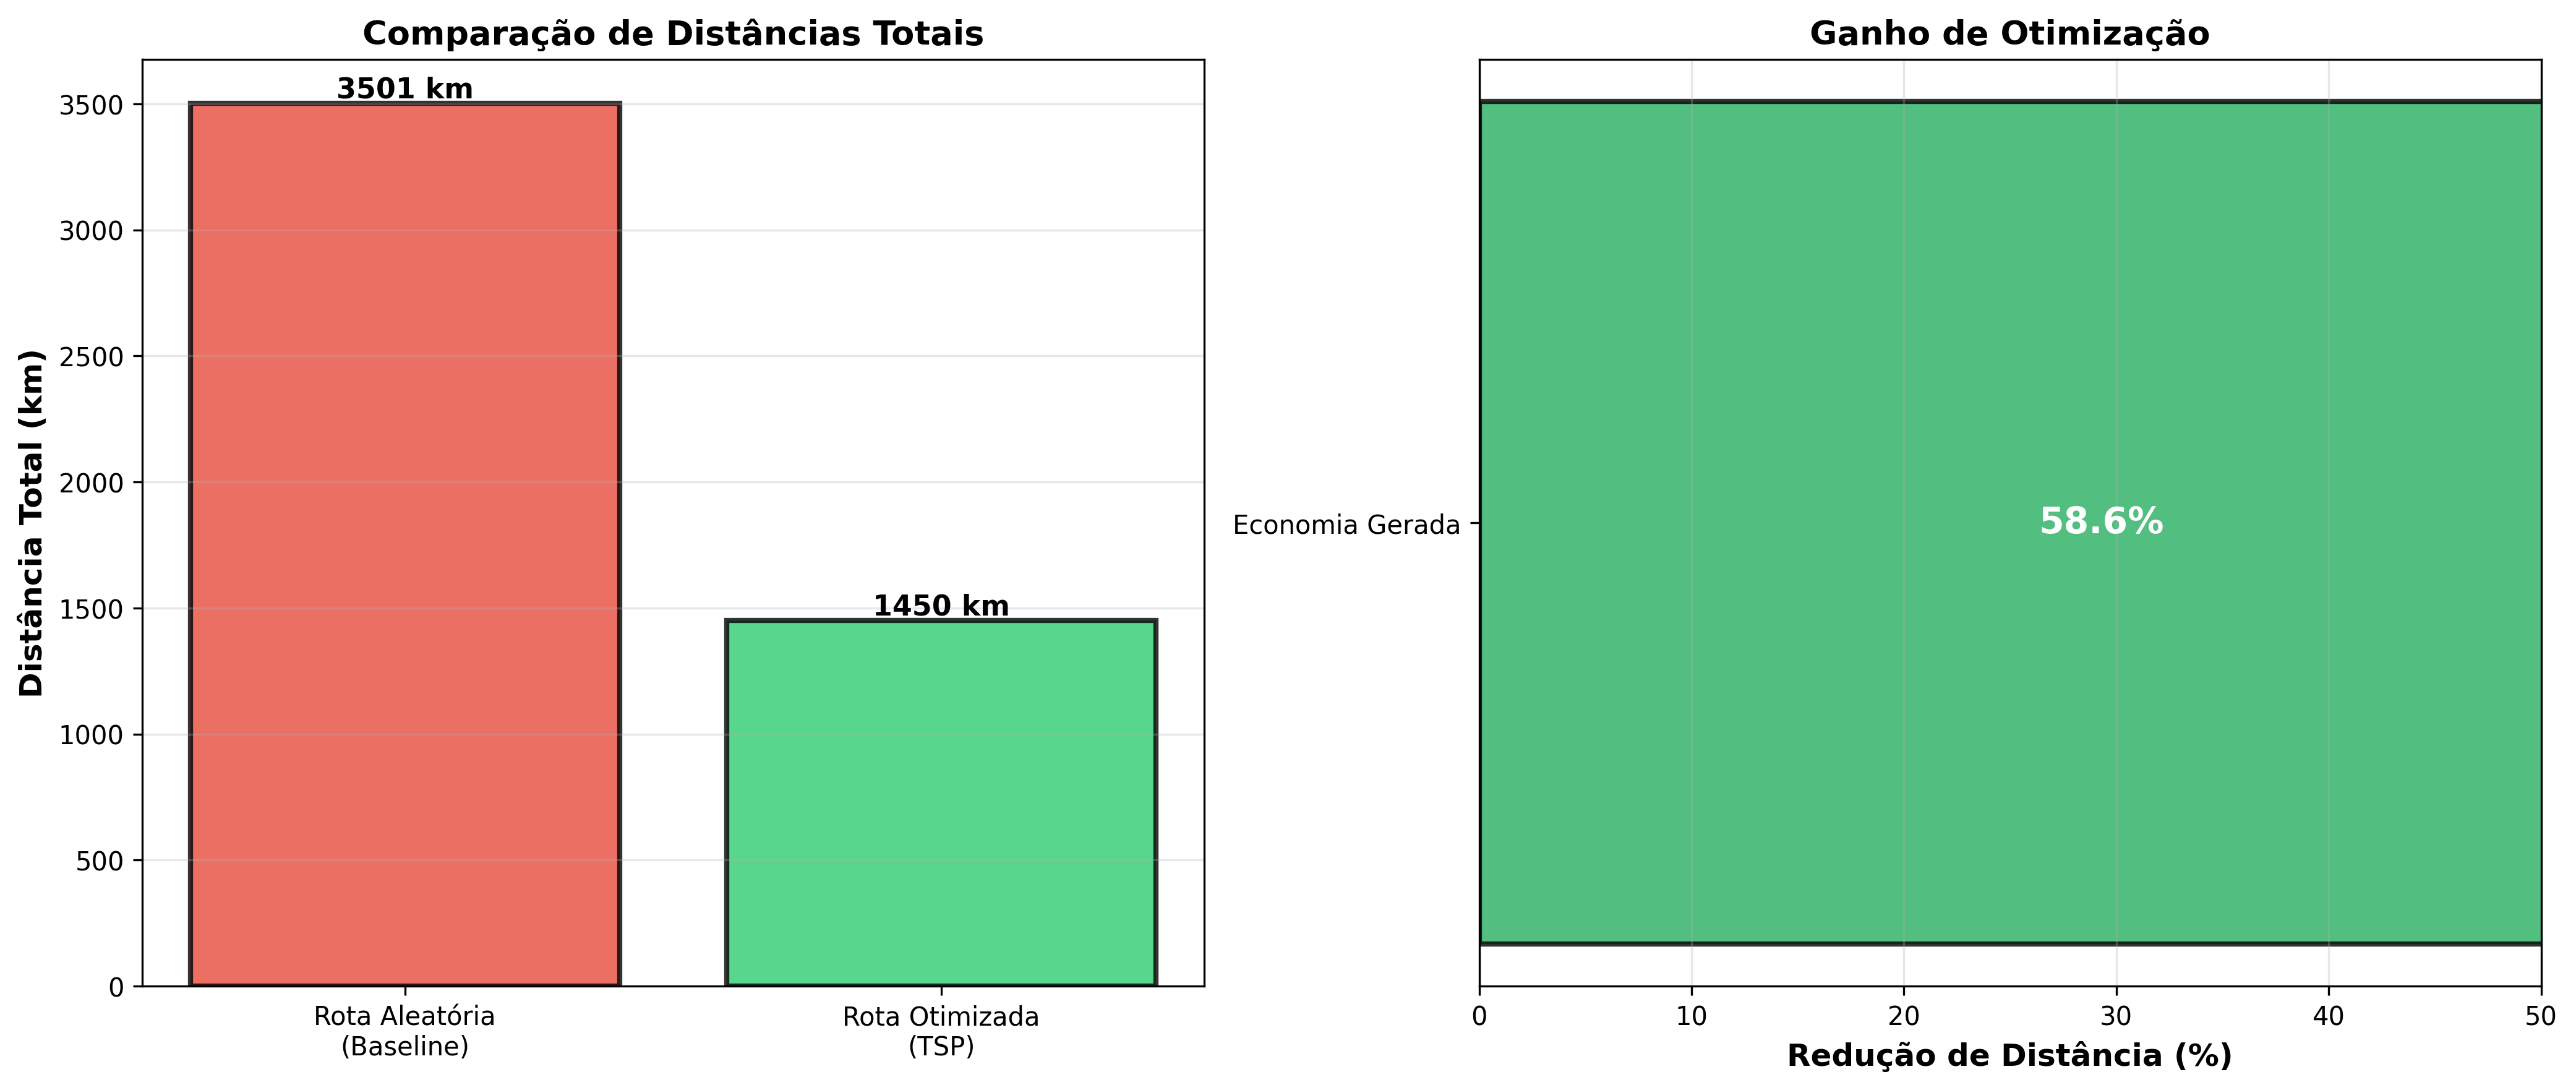
\includegraphics[width=0.9\textwidth]{comparativo_master.png}
\caption{Comparativo de distâncias totais e economia percentual}
\label{fig:comparativo_master}
\end{figure}

\subsection{Distribuição de Impressoras}

A Figura~\ref{fig:distribuicao} ilustra a distribuição de volumetria por cidade.

\begin{figure}[H]
\centering
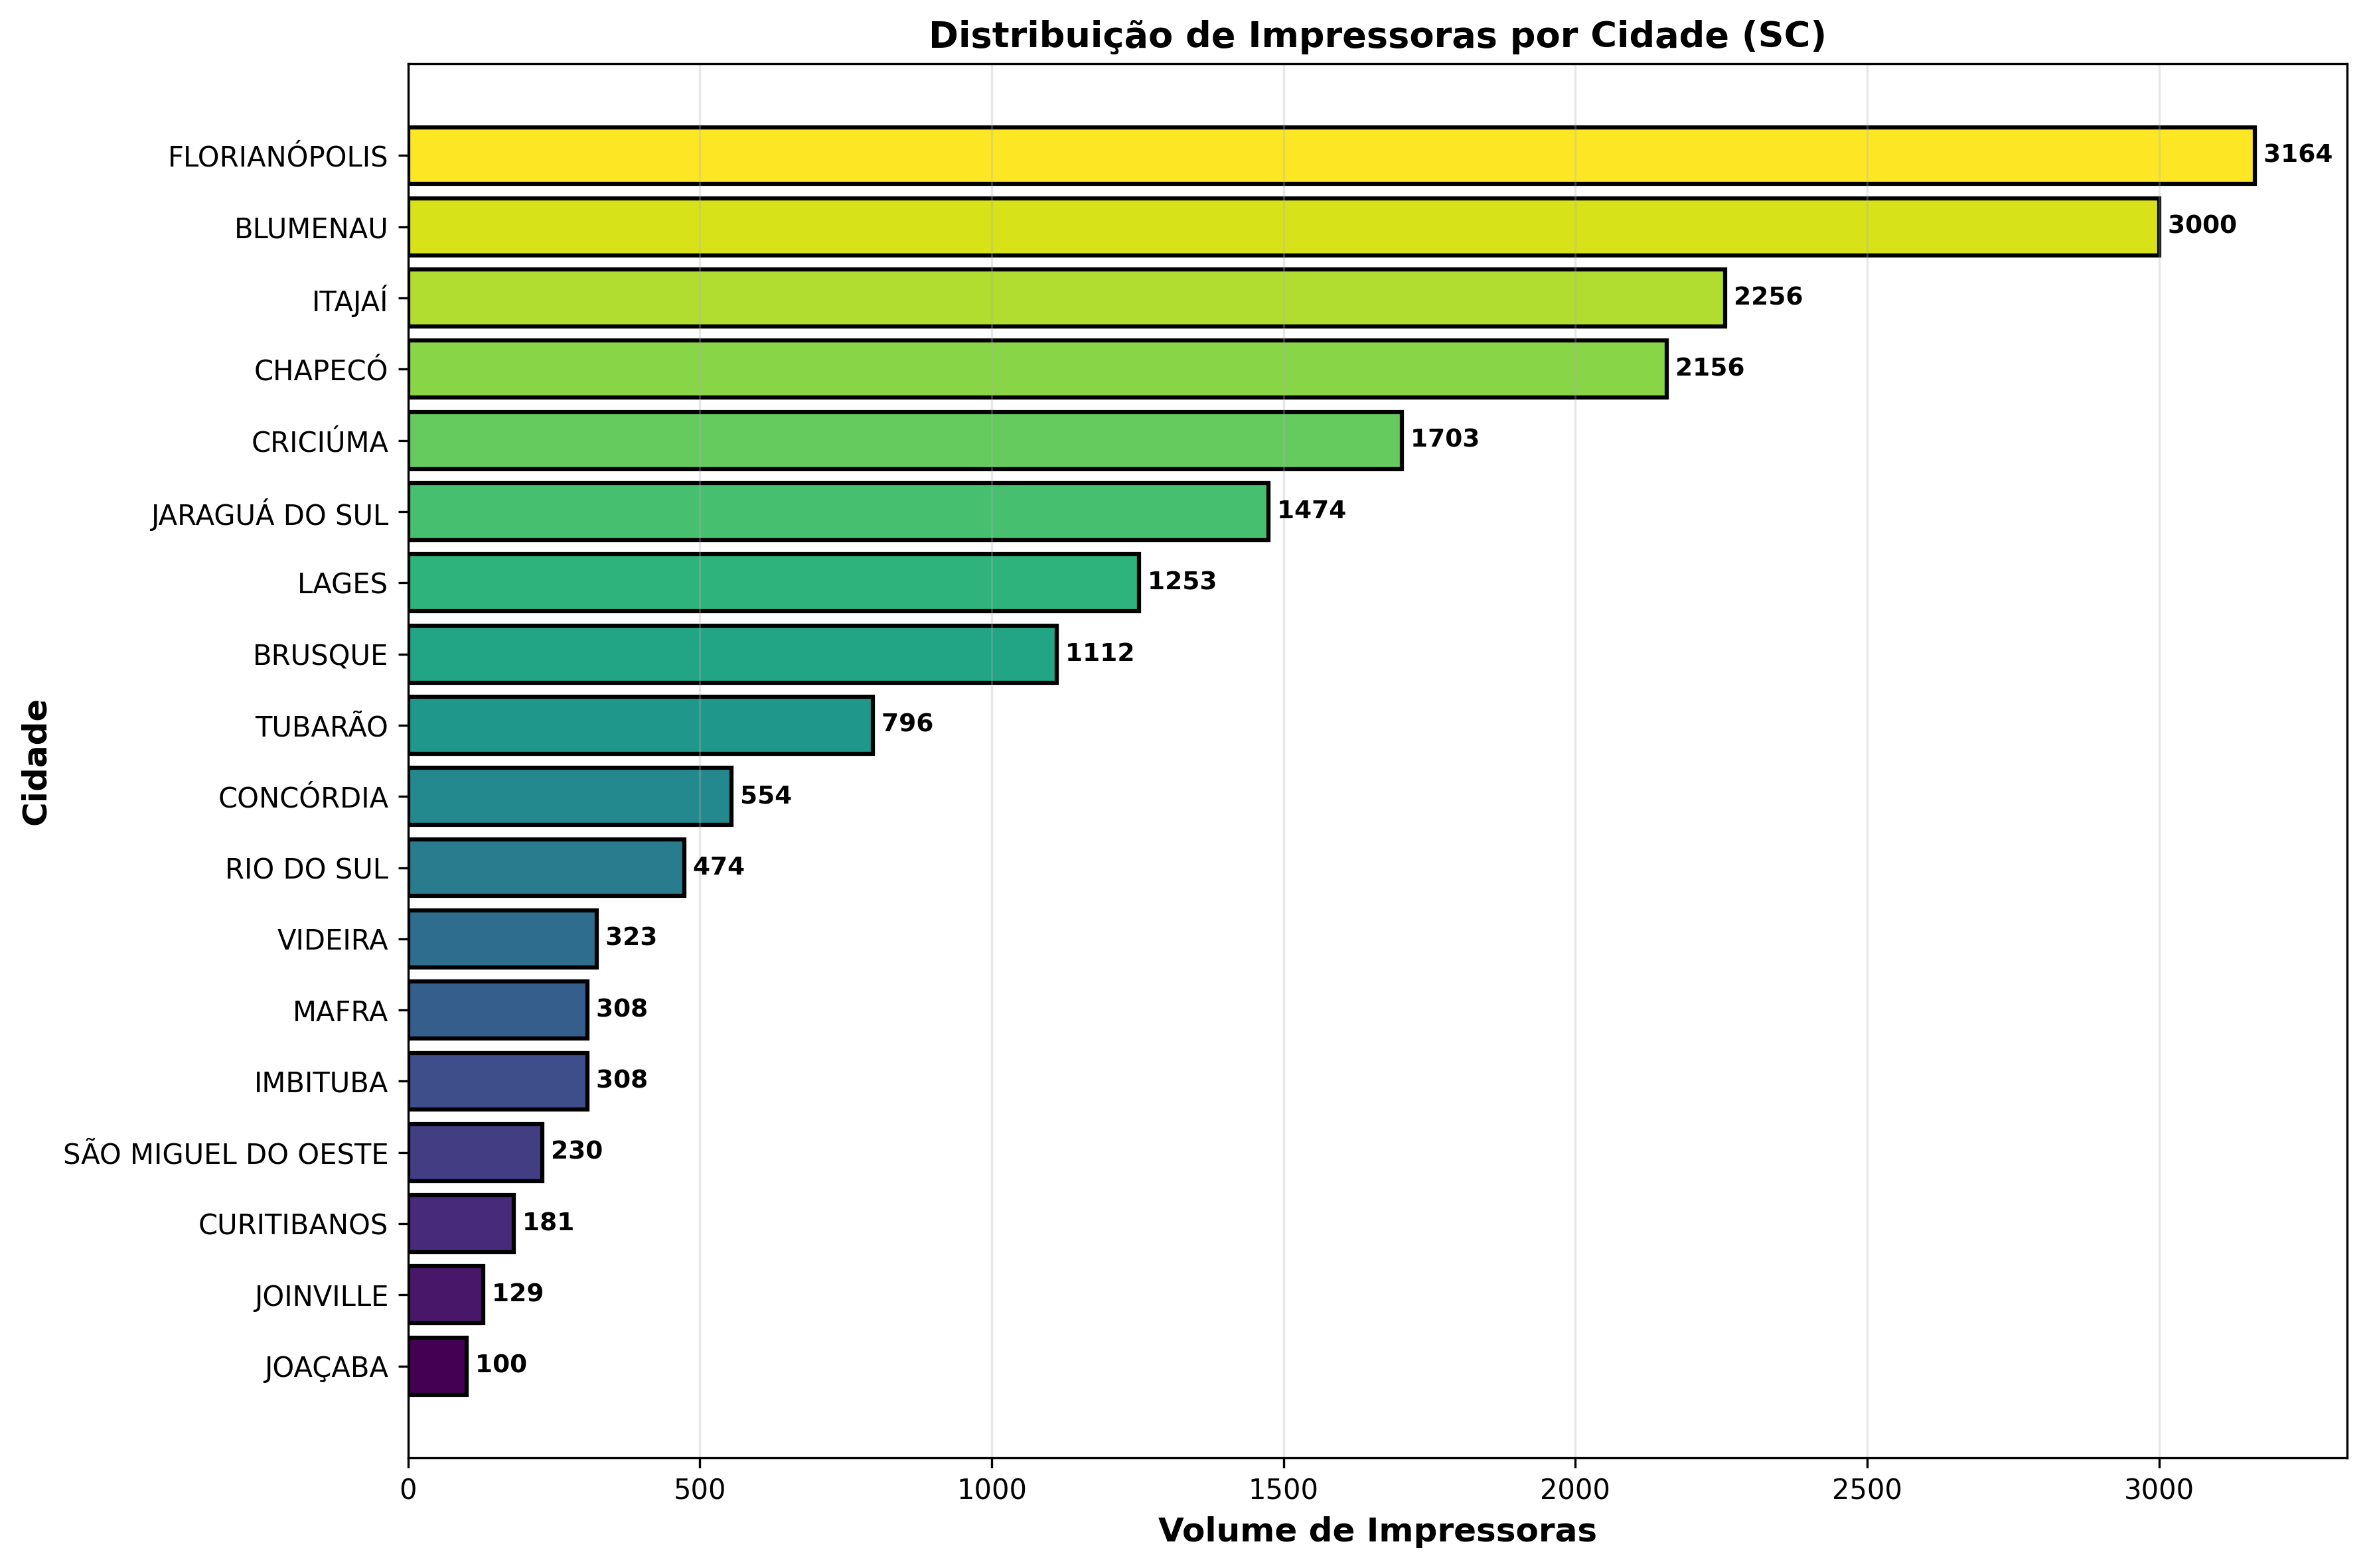
\includegraphics[width=0.9\textwidth]{distribuicao_impressoras.png}
\caption{Distribuição de impressoras por cidade em Santa Catarina}
\label{fig:distribuicao}
\end{figure}

\section{Conclusão}

O algoritmo de otimização de rotas (Nearest Neighbor + 2-opt) alcançou uma
redução de \textbf{58.58\%%} na distância total percorrida, resultando em 
\textbf{2.41 vezes} mais eficiência logística.

\end{document}
